\section{Realtime planlægning i \pycsp}
\label{sec:rtp-pycsp}
\fxnote{(Flyttet fra RTP overordnet) Husk at snakke om begrænsning af greenlets mht. parallelitet når vi arbejder i realtid}
Da vi ønsker at introducere RTP i \pycsp, er der er række forhold, som vi skal tage højde for. Vi vil i dette afsnit tage udgangspunkt i de ovenstående opstillede muligheder og sammenholde dem med \pycsp. 

I \pycsp kan vi anskue processerne som begivenheder og derved bruge skemaplanlæggeren i \code{greenlets}-versionen til at styre hvilken proces og dermed hvilken begivenhed, der udføres. Vi har ikke umiddelbart informationer om, hvor lang tid en proces er om at blive udført, og det vil kræve en analyse af den enkelte proces at udlede estimater for det. Vi har valgt at fokusere på selve planlægningen af processerne og ikke på analysen. Dermed har vi ikke mulighed for at benytte RM og LL algoritmerne, da de begge benytter information om udførselstiden for en proces. Derved har vi EDF tilbage som mulighed, hvilket vi i det følgende vil implementere. En udvidelse af \pycsp til at benytte EDF er forholdsvis ligetil. Der skal laves en mulighed for, at brugeren kan angive en deadline til en proces, og vi skal ved kontekstskift sikre, at vi aktiverer den proces, der har den førstkomne deadline. Såfremt en deadline overskrides, skal vi have funktionalitet, til at håndtere dette. 
I forbindelse med kommunikation, skal vi se hvordan processer med deadlines bliver påvirket af  any-to-any kanalerne og det prioriterede valg i \code{alternation}.

Den eneste form for intern afhængighed der findes mellem processer i \pycsp er per definition i forbindelse med kommunikation over kanaler, og vi kan derfor opleve problemer med prioritetsinvertering. Den eneste metode til håndtering af dette, der kan bruges sammen med \pycsp, er prioritetsnedarvning, da de andre metoder forudsætter prioritetsinverteringen  sker som resultat af tilgang til kritiske regioner og ikke pga. kommunikation. Vi skal derfor også implementere prioritetsnedarvning for at sikre os mod prioritetsinvertering. 

Da vi benytter os af \code{greenlets}-versionen af \pycsp arbejder vi med en skemaplanlægger, der ikke kan foretage preemptive kontekstskift. Dette kan lede til problemstillinger som det er illustreret på \cref{fig:edf-nonpreemptive}. En metode til at mindske denne type problemer er at lade de enkelte processer afgive kontrollen med jævne mellemrum. Herved vil der blive foretaget en ny evaluering af hvilken proces, der skal aktiveres, og hvis der er processer, der har en nærmere deadline, som er blevet klar, aktiveres en af disse. Dette beror helt og holdent på at hver enkelt proces frivilligt afgiver kontrollen og gør det med jævne mellemrum, når den er aktiv. Dette betyder, at det er overladt til udvikleren at indsætte det på relevante steder i processens kode. 

\subsection{Tilknytning og overskridelse af deadlines}
Som udgangspunkt skal vi kunne håndtere, at en proces kan have forskellige typer deadlines. Umiddelbart er det oplagt, at der for hver proces tilknyttes en deadline samt hvilken type, det er. Dette giver mulighed for, at vi kan differentiere i den måde vi håndterer en overskreden deadline. F.eks. kan vi stoppe systemet helt i tilfælde af overskridelse af en kritisk deadline, kaste en exception ved en hard deadline og blot registrere overskridelser af soft deadlines. Uanset hvilken handling vi vælger at tilknytte til de respektive overskridelser, vil der altid være situationer, hvor den valgte handling ikke er optimal. 

Vi har derfor valgt en anden løsning, hvor en proces blot kaster en exception, hvis den overskrider en deadline. Dette overflødiggør, at der tilknyttes en specifik type deadline til en proces, da håndteringen af den kastede exception overgives til udvikleren. Det er herved op til den enkelte udvikler at definere, hvad der skal ske i hver enkelt proces, såfremt den overskrider en deadline. Dette giver den største frihed til at tilpasse håndteringen til den enkelte proces og applikation. 

\subsection{Udvælgelse af proces}
Udvælgelsen af hvilken proces der skal aktiveres, ved et kontekstskift, er givet ud fra vores valg af EDF. Som beskrevet i \cref{sec:edf} specificerer EDF, at det altid processen med den nærmeste deadline der skal aktiveres. For at opnå dette kan vi benytte stort set samme metode som vi brugte i \des. I \des sorterede vi processerne efter hvilket tidskridt de skulle aktiveres i, her kan vi sortere dem ud fra deres deadline.  

\subsection{Kanalkommunikation}\label{sec:rtp-kommunikation}
I litteraturen for  RTP fokuseres der kun på udvælgelsen og planlægningen af processer i \sched en. I \pycsp er kommunikation blokerende, hvilket betyder at en proces er  blokeret fra den ønsker at kommunikere, til kommunikationen er gennemført. Ved one-to-one kanaler, er der kun en proces i hver ende, og derfor er  processen garanteret at gennemføre kommunikationen når modparten er klar til at kommunikere. Har processerne forskellige prioriteter risikere man prioritetsinvertering, og kan afhjælpe det med prioritetsnedarvning. 

I \pycsp er one-to-one kanalerne blevet fjernet, og erstattet af any-to-any kanaler, der ud fra et teknisk synspunkt er mere generelle og kan alt som one-to-one kanalerne kan. I any-to-any kanalerne er man ikke begrænset til kun at have en proces i hver ende af kanalen, men der kan være et vilkårligt antal processer. 
Benyttes prioritetsnedarvning på any-to-any kanaler, er man ikke som ved one-to-one kanaler sikret at det processen der startede  prioritetsnedarvningen der får gavn af den, da parringen mellem processer der ønsker at kommunikere sker tilfældigt. Når processer kommunikerer i any-to-any kanaler ønsker vi at det altid er den proces med højst prioritet der kommer til at kommunikere, for at ahjælpe problemet med den tilfældige parring af processerne. 


\subsection{Prioritetsnedarvning}\label{sec:rtp-pycsp-nedarvning}
At introducere prioritetsnedarvning i \pycsp virker umiddelbart ligetil, idet vi kan se de indbyrdes afhængigheder klart ud fra forbindelserne gennem kanalerne. Der kan forekomme andre afhængigheder, som er mindre synlige, men vi mener ikke disse vil forekomme i velskrevne CSP applikationer, og vi har derfor valgt at begrænse os til afhængigheder repræsenteret vha. kanaler. På trods af den umiddelbare simplicitet skal vi overveje hvornår, hvem og hvor længe, der skal arves i forbindelse med prioritetsnedarvning.

\subsubsection{Ændring af prioritet}
\label{sec:aendring-af-prioritet}
Vi arbejder med et dynamisk system af processer, hvor en proces, på baggrund af sin tilstand, er afhængig af forskellige andre processer for at kunne arbejde videre. 
Hvis vi højner prioriteten på alle processer, der er forbundet til en proces med høj prioritet, vil mange af processerne, der arver den høje prioritet, reelt ikke kunne bidrage til udførelsen af den proces, der starter med høj prioritet. Det er en bedre løsning, at det kun er den eller de processer, der kan sikre videre udførsel af den aktuelle proces, der tildeles højere prioritet. Hvis eksempelvis en proces med høj prioritet ønsker at skrive på en kanal, skal alle processer, der læser på den kanal, arve den høje prioritet, men de processer, som ønsker at skrive til en anden kanal, som processen med høj prioritet læser fra, ikke skal arve den høje prioritet. Generelt set betyder det, at der kun skal udføres prioritetsnedarvning, såfremt en højt prioriteret proces venter på at kommunikere, såfremt der ikke er andre processer, der er klar til at indgå i den ønskede kommunikation. 

Vi har nu begrænset os til, at det kun er de processer der kan indgå i kommunikation over en kanal, der arver en prioritet. Med any-to-any kanaler findes der dog et vilkårligt antal processer i hver kanalende, og man risikerer en prioritetsdevaluering ved at lade flere processer arve en høj prioritet. I klassisk \csp findes der modsat hertil one-to-one kanaler, hvor man er sikret at det kun én proces' prioritet der bliver højnet ved prioritetsnedarvning. Forskellen illustreres af \autoref{fig:one-to-one-inheritance} og \cref{fig:any-to-any-inheritance}\fxerror{tjek sidenr. er korrekt for de to figurer inden aflevering}. På \autoref{fig:one-to-one-inheritance}, bliver en proces' prioritet hævet fra fem til 10. Modtageren kan uden afbrydelser arbejde hen mod at kunne kommunikere, da afsenderen venter. I \autoref{fig:any-to-any-inheritance} bliver alle tre processers prioritet hævet til 10 og de vil skulle kæmpe mod hinanden for komme frem til en tilstand hvor de ønsker at kommunikere. 

\begin{figure}
 \begin{center}
  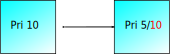
\includegraphics[scale=1.00]{images/one-to-one-inheritance}
\caption{Procesnetværk med en afsender og en modtager. Afsenderen har prioritet 10, mens modtageren har en initiel prioritet på fem. Modtageren  får via prioritetsnedarvning hævet sin prioritet til 10. (Højere er bedre)}
  \label{fig:one-to-one-inheritance}
  \end{center}
\end{figure}

\begin{figure}
 \begin{center}
  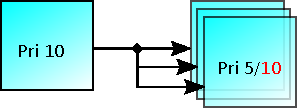
\includegraphics[scale=1.00]{images/any-to-any-inheritance}
  \caption{I dette eksempel findes der tre modtagere, som alle får hævet deres prioritet til 10.}
  \label{fig:any-to-any-inheritance}
  \end{center}
\end{figure}

Prioritetsnedarvning i et miljø med any-to-any kanaler har dermed en risiko for at medføre prioritetsdevaluering. Man kan forstille sig forskellige metoder til at eliminere eller minimere problemet f.eks ved at begrænse antallet af processer, der kan modtage en prioritetsnedarvning. Dette kunne gøres ved kun at lade en enkelt proces arve prioriteten,  men så skal man tage stilling til, hvilken proces, der skal udvælges. Dette kunne være den proces, der er tættest på at indgå i kommunikationen.  Udvælgelsen af processer må dog bero på en analyse af den enkelte applikation og dens aktuelle tilstand. Da vi ikke ønsker at begynde på en analyse af udviklerens kode, må vi nødvendigvis sende prioritetsnedarvningen til alle processerne på kanalen. For at løse problemet vil vi i stedet fokusere på at minimere antallet af processer, der starter prioritetsnedarvningen, og det tidsrum processerne har arvet en prioritet.

Når kommunikationen på kanalen er gennemført, befinder processens sig i en anden tilstand og er afhængig af noget andet for at komme videre i sin udførsel. 
Når det midlertidige afhængighedsforhold ophører skal processer der har arvet en prioritet miste denne. Der skal selvfølgelig tages højde for at en proces kan arve forskellige prioriteter fra forskellige andre processer, så det skal være muligt at falde tilbage til den næsthøjeste arvede prioritet, i stedet for blot at skifte tilbage til den oprindelige prioritet. 

\subsection{Alternation}\label{misc:kanal-prioritet}
Det er dog ikke kun i forbindelse med almindelig kommunikation vi skal forholde os til introduktionen af processer med prioritet. I kodestrukturen \code{alternation}
har en udvikler mulighed for at foretage et  prioriteret valg mellem flere forskellige kanaler. Et prioriteret valg mellem flere kanaler, kan dog være i konflikt med de processer som får opfyldt deres kommunikation\fxwarning{Denne sætning giver ikke mening}
  
\citeauthor{Burns1990} beskriver og illustrerer præcist denne problemstilling i \citetitle{Burns1990}\cite{Burns1990}. Til at illustrere problemet beskriver de et eksempel, som er vist i \cref{lst:pri-select}. Denne kodestump viser et prioriteret valg mellem kanalerne A1 og A2. Til hver kanal er tilknyttet en proces, P1 og P2. Disse to processer har en prioritet tilknyttet på hhv.  Pri1 og Pri2. \CRef{tab:prioritizedSelect} viser hvilken kanal der bliver valgt, afhængig af processernes prioritet.

\begin{lstlisting}[firstnumber=1 ,float=hbtp, label=lst:pri-select, caption={(priority) select. Eksemplet er kopieret fra \cite{Burns1990}}]
(priority) select
   A1 -- Process P1
 or
   A2 -- Process P2
 end select
\end{lstlisting}

\begin{table}[htbp]
	\centering
	\begin{tabular}{lccc}
       	\toprule
                        & Pri1 > Pri2 & Pri1 = Pri2 & Pri1 < Pri2\\
        \midrule
	    priority select & A1          & A1          & ?  \\
        \bottomrule
        \end{tabular}
    \caption[]{Konflikten ved brug af prioriteret valg og procesprioriteter. Eksemplet er kopieret fra \cite[160]{Burns1990}}\\
    \label{tab:prioritizedSelect}
\end{table}

Man kan af \cref{tab:prioritizedSelect}  konstatere at der opstår en konflikt i kolonne tre, hvis udvikleren foretrækker en kanal, hvor den  tilknyttede proces' prioritet er lavere  end den anden proces'  prioritet. Man vil ikke kunne opfylde begge krav om både at kommunikere med den proces med højst prioritet, og lade udvikleren bestemme kanalen. For \citeauthor{Burns1990} er løsningen en ``orthogonal solution'', der håndterer begge typer prioriteter. De ønsker overordnet set to typer udvælgelsesmetoder, weak- og strong Select. Weak select sorterer primært efter processernes prioritet og sekundært efter det prioriterede valg. Strong select udvælger udelukkende processer efter det prioriterede valg. De forstiller sig, at weak select skal bruges som den primære metode, men i specielle tilfælde skal en udvikler have mulighed for at tvinge et prioriteret valg igennem.

I artiklen fra \citeauthor{Burns1990} har de kun beskæftiget sig med one-to-one kanaler, og det er denne antagelse der medfører at et valg af kanal medfører et valg af en proces og dennes prioritet. Dette er ikke en mulighed i \pycsp hvor kanalerne er af typen any-to-any. Et valg af en kanal, medfører derfor ikke en direkte kobling til en proces, men til vilkårligt mange processer, der kan have individuelle  prioriteter. I \cref{sec:rtp-kommunikation} kommer vi frem til at kommunikationen altid skal sørge for at det er den højst prioriterede proces der kommunikerer. Dette kan bruges i \code{alternation} til at finde den højst prioriterede proces, for hver kanal, der er klar til at kommunikere og udvælge den kanal der har den højst prioriterede proces. 

På baggrund af artiklen har vi valgt at \code{alternations} udfører en weak select, da denne version egner sig bedst til RTP . Vi vil i vores version ikke inkludere en strong select. Dette gør vi ud fra en betragtning om at den kun bør bruges i sjældne tilfælde,  da den vil modarbejde ideen bag RTP. Hvis en udvikler alligevel ønsker denne funktionalitet, vil han godt kunne opnå det i \pycsp, men vi ønsker ikke at tilskynde dette, ved inkludere det i RTP versionen af \pycsp.

\subsubsection{Prioritetsnedarvning i \code{alternation}}
Vi har som nævnt i \cref{sec:rtp-pycsp-nedarvning} en klar kæde af afhængigheder i \pycsp, men vi skal være opmærksomme på ikke at højne processers prioritet unødigt i forbindelse med prioritetsnedarvning. Dette kan let blive tilfældet såfremt vi ikke holder ordentligt styr på, hvorfor en proces har den prioritet, den har, om den er sat af udvikleren, eller den er nedarvet. Man kan forestille sig en situation, hvor et uddrag af et proces-neværk består af en generator-forbruger-model med to generatorer og en enkelt forbruger. De to generatorer er forbundet til forbrugeren vha. en \code{alternation}, og har henholdsvis høj og lav prioritet. Eksemplet er illustreret på \cref{fig:alt-inheritance}. Forbrugeren vil i dette scenarium arve den høje prioritet fra den tilsvarende generator, men utilsigtet vil den høje prioritet derefter også propagere fra forbrugeren til generatoren med lav prioritet. Dette er ikke hensigtsmæssigt, da de to generatorer nu har lige høj prioritet og ikke det forhold, som udvikleren oprindeligt har angivet. Vi kan dog indse, at dette ikke bliver et problem, idet vi kun udfører prioritetsnedarvning i det tilfælde, hvor der ikke er nogen processer, der er er klar til at indgå i ønsket kommunikation. I det opstillede tilfælde vil forbrugeren derfor ikke foretage yderligere prioritetsnedarvning på generatoren med lav prioritet, da generatoren med høj prioritet altid vil være klar til at skrive i denne situation. 

\begin{figure}
 \begin{center}
  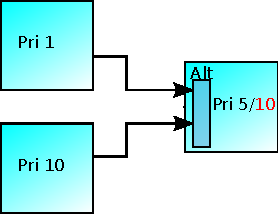
\includegraphics[scale=1.00]{images/alt-inheritance}
  \caption{Prioritetsnedarvning i \code{alternations.}}
  \label{fig:alt-inheritance}
  \end{center}
\end{figure}
